\documentclass{beamer}
\title{Introduction to Functional Programming with Haskell - RCOS Presentation}
\date{February 27, 2015}
\author{Avi Weinstock}
%\usepackage{listings}
%\lstset{language=Haskell}
%\usepackage{framed}
\usepackage{fancyvrb}
\begin{document}
\maketitle

\begin{frame}
\frametitle{What characterizes Functional Programming?}
\begin{itemize}
\item
Abstraction of common patterns via higher order functions
\item
A mathematical use of the term "function" (as a pure mapping from input to output), as opposed to the concept of procedures (e.g. in C)
\end{itemize}

\end{frame}
\begin{frame}
\frametitle{What is Haskell?}
A general-purpose programming language that:
\begin{itemize}
\item
Encourages a functional style of programming
\item
Enables very short, readable code
\item
Has static typechecking, with type inference
\item
Compiles to native code, in the same efficiency class as Java/C\# (can be made as performant as Assembly/C/C++, with some effort)
\end{itemize}
\end{frame}

\begin{frame}[fragile]
\frametitle{Hello world}
%Functions introduced:
%\begin{Verbatim}[frame=single, fontsize=\scriptsize]
%getLine :: IO String
%interact :: (String -> String) -> IO ()
%\end{Verbatim}
%Examples:
\begin{itemize}
\item
\begin{Verbatim}[frame=single, fontsize=\scriptsize]
main = putStrLn "Hello, world!"
\end{Verbatim}
\item
\begin{Verbatim}[frame=single, fontsize=\scriptsize]
main = do
    putStr "Enter a string: "
    str <- getLine
    putStrLn ("Echo: " ++ str)
\end{Verbatim}
%\item
%\begin{Verbatim}[frame=single, fontsize=\scriptsize]
%import Network
%main = do
%    sock <- listenOn (PortNumber 8000)
%    
%\end{Verbatim}
\end{itemize}
\end{frame}

\begin{frame}[fragile]
\frametitle{Examples with numbers}
\begin{itemize}
\item
\begin{Verbatim}[frame=single, fontsize=\scriptsize]
factorial n = product [1..n]
\end{Verbatim}
\item
\begin{Verbatim}[frame=single, fontsize=\scriptsize]
dotProduct xs ys = sum $ zipWith (*) xs ys
dotProduct' xs ys = sum (zipWith (*) xs ys) -- equivalent definition
magnitude xs = sqrt $ dotProduct xs xs
\end{Verbatim}
\item
\begin{Verbatim}[frame=single, fontsize=\scriptsize]
divides n i = (n `mod` i) == 0
isPrime n = not $ any (divides n) [1..n]
isPrime' n = not (any (divides n) [1..n]) -- equivalent definition
\end{Verbatim}
\end{itemize}
%ghci -XNoMonomorphismRestriction
%:set prompt "ghci> "
%:load haskell_lecture_numberslide.hs
%:browse
%map factorial [1..10]
%magnitude [1,1]
%take 10 $ filter isPrime [2..]
%take 10 fibonaccis
%plot (^2) [0..7]
%plot (approxDerivative 0.01 (^2)) [0..7]
\end{frame}

\begin{frame}[fragile]
\frametitle{Examples with numbers (continued)}
\begin{itemize}
\item
\begin{Verbatim}[frame=single, fontsize=\scriptsize]
fibonaccis = 1 : 1 : zipWith (+) fibonaccis (tail fibonaccis)
\end{Verbatim}
\item
\begin{Verbatim}[frame=single, fontsize=\scriptsize]
approxDerivative epsilon f x = (f (x+epsilon) - f x) / epsilon
\end{Verbatim}
\item
\begin{Verbatim}[frame=single, fontsize=\scriptsize]
stars n = replicate (floor n) '*'
showLines = putStr . unlines
prepend = zipWith ((++) . show)
plot f xs = showLines $ prepend xs (map (stars . f) xs)
\end{Verbatim}
\end{itemize}
\end{frame}

\begin{frame}[fragile]
\frametitle{Execution of examples}
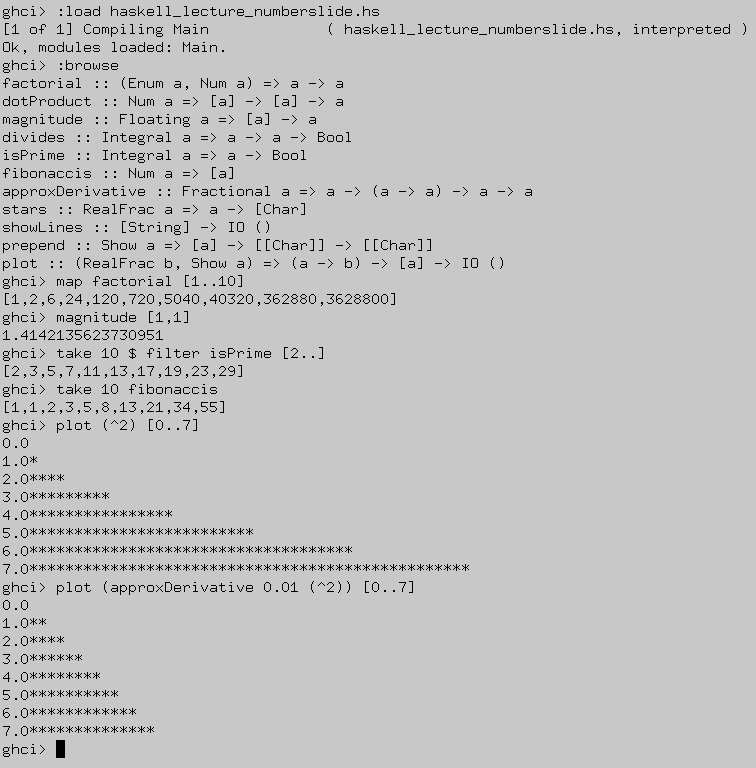
\includegraphics[scale=0.25]{haskell_lecture_numberslide_ghci1_cropped.png}
\end{frame}

\begin{frame}[fragile]
\frametitle{Functions used in previous examples}
\begin{Verbatim}[frame=single, fontsize=\scriptsize]
($) :: (a -> b) -> a -> b
f $ x = f x

(.) :: (b -> c) -> (a -> b) -> (a -> c)
(f . g) x = f (g x)

not :: Bool -> Bool
any, all :: (a -> Bool) -> [a] -> Bool

zip :: [a] -> [b] -> [(a, b)]
zipWith :: (a -> b -> c) -> [a] -> [b] -> [c]

sum, product :: Num a => [a] -> a

replicate :: Int -> a -> [a]

putStr, putStrLn :: String -> IO ()
\end{Verbatim}
\end{frame}

\begin{frame}[fragile]
\frametitle{Map and Reduce}
\begin{Verbatim}[frame=single, fontsize=\scriptsize]
map :: (a -> b) -> [a] -> [b]
map f [] = []
map f (x:xs) = (f x):(map f xs)

map' f = foldr ((:) . f) [] -- equivalent definition

foldr :: (a -> b -> b) -> b -> [a] -> b
foldr f acc [] = acc
foldr f acc (x:xs) = f x (foldr f acc xs)
\end{Verbatim}
\verb|map| applies its function to every element of a list.\\
\verb|foldr| uses the provided function to reduce/aggregate the list into some value, starting from a seed.\\
Folds are very general, and can be used to implement many types of loops.\\
Definition of \verb|foldl| in Python:
\begin{Verbatim}[frame=single, fontsize=\scriptsize]
def foldl(f, init, xs):
    acc = init
    for x in xs:
        acc = f(acc, init)
    return acc
\end{Verbatim}
\end{frame}

\begin{frame}[fragile]
\frametitle{Reduce (continued)}
More definitions of things in terms of \verb|foldr|:
\begin{Verbatim}[frame=single, fontsize=\scriptsize]
map f = foldr ((:) . f) []

sum = foldr (+) 0

product = foldr (*) 1

concat = foldr (++) []

all p = foldr ((&&) . p) True

any p = foldr ((||) . p) False
\end{Verbatim}
\end{frame}

\begin{frame}[fragile]
\frametitle{Typeclasses}
With this definition:
\begin{Verbatim}[frame=single, fontsize=\scriptsize]
instance Num a => Num [a] where
    (+) = zipWith (+)
    (*) = zipWith (*)
    (-) = zipWith (-)
    negate = map negate
    abs = map abs
    signum = map signum
    fromInteger = cycle . return . fromInteger
\end{Verbatim}
Expressions like these become valid:
\begin{Verbatim}[frame=single, fontsize=\scriptsize]
1 + [1,2,3]
2 * [2..10]
-[6,2,8]
abs [-5..5]
\end{Verbatim}
\end{frame}

\begin{frame}[fragile]
\frametitle{Currying, Sections, and Infix}
The following are all equivalent (via currying):
\begin{Verbatim}[frame=single, fontsize=\scriptsize]
f g x y = zipWith g x y
f g x = zipWith g x
f g = zipWith g
f = zipWith
f g x = \y -> zipWith g x y
f g = \x y -> zipWith g x y
f = \g x y -> zipWith g x y
\end{Verbatim}
These are equivalent triples (via sections, and infix):
\begin{Verbatim}[frame=single, fontsize=\scriptsize]
g x = x + 1
g = (+1)
g x = (+) x 1
\end{Verbatim}
\begin{Verbatim}[frame=single, fontsize=\scriptsize]
h x = x `mod` 2
h = (`mod` 2)
h x = mod x 2
\end{Verbatim}
\begin{Verbatim}[frame=single, fontsize=\scriptsize]
i x = 2 `mod` x
i = (2 `mod`)
i x = mod 2 x
\end{Verbatim}
Note that $\verb|h| \neq \verb|i|$, since \verb|mod| is not commutative.
\end{frame}

\begin{frame}[fragile]
\frametitle{TIMTOWTDI - There's More Than One Way To Do It}
Functions introduced:
\begin{Verbatim}[frame=single, fontsize=\scriptsize]
ord :: Char -> Int
chr :: Int -> Char

interact :: (String -> String) -> IO ()

forever :: Monad m => m a -> m b
\end{Verbatim}
\begin{Verbatim}[frame=single, fontsize=\scriptsize]
import Control.Monad
import Data.Char

caesarCipher shift = map (chr . (`mod` 256) . (+ shift) . ord)

main1 = forever $ do
    plaintext <- getLine
    let ciphertext = caesarCipher 3 plaintext
    putStrLn (caesarCipher 3 plaintext)

main2 = forever (getLine >>= (putStrLn . caesarCipher 3))

main3 = interact (caesarCipher 3)
\end{Verbatim}
\end{frame}

\begin{frame}[fragile]
\frametitle{Binary Search Trees}
\begin{Verbatim}[frame=single, fontsize=\scriptsize]
{-# LANGUAGE NoMonomorphismRestriction #-}
import Data.Foldable as F

data BinaryTree a = Node a (BinaryTree a) (BinaryTree a) | Empty
    deriving (Eq, Show, Ord)

instance Foldable BinaryTree where
    foldr f acc Empty = acc
    foldr f acc (Node x l r) = F.foldr f (f x (F.foldr f acc r)) l

treeInsert x Empty = Node x Empty Empty
treeInsert x (Node y l r) = case compare x y of
    LT -> Node y (treeInsert x l) r
    GT -> Node y l (treeInsert x r)
    EQ -> Node y l r

treeFind x Empty = Empty
treeFind x (Node y l r) = case compare x y of
    LT -> treeFind x l
    GT -> treeFind x r
    EQ -> Node y l r
\end{Verbatim}
\end{frame}

\begin{frame}[fragile]
\frametitle{Binary Search Trees (continued)}
\begin{Verbatim}[frame=single, fontsize=\scriptsize]
treeRemove x Empty = Empty
treeRemove x (Node y l r) = case compare x y of
    LT -> Node y (treeRemove x l) r
    GT -> Node y l (treeRemove x r)
    EQ -> case (l, r) of
        (Empty, Empty) -> Empty
        (_, Empty) -> l
        (Empty, _) -> r
        (_, _) -> let lMax = F.maximum l in
            Node lMax (treeRemove lMax l) r 
\end{Verbatim}
\end{frame}

\begin{frame}[fragile]
\frametitle{Quicksort}
\begin{Verbatim}[frame=single, fontsize=\scriptsize]
{-# LANGUAGE NoMonomorphismRestriction #-}
import Control.Monad
import Control.Monad.ST
import Data.STRef
import qualified Data.Vector as V
import qualified Data.Vector.Mutable as VM

import Data.List
import Test.QuickCheck

partitionByST cmp vec lo hi = VM.read vec pivotIdx >>= aux lo lo hi where
    pivotIdx = lo + ((hi-lo) `div` 2)
    aux i j n mid | j <= n = do
        a_j <- VM.read vec j
        case cmp a_j mid of
            LT -> VM.swap vec i j >> aux (i+1) (j+1) n mid
            GT -> VM.swap vec j n >> aux i j (n-1) mid
            EQ -> aux i (j+1) n mid
    aux i j n mid = return (i, j)
\end{Verbatim}
\end{frame}

\begin{frame}[fragile]
\frametitle{Quicksort (continued)}
\begin{Verbatim}[frame=single, fontsize=\scriptsize]
quicksortByST cmp vec = aux 0 (VM.length vec - 1) where
    aux lo hi = when (lo < hi) $ do
        (leftMid, rightMid) <- partitionByST cmp vec lo hi
        aux lo leftMid
        aux rightMid hi

quicksortBy cmp vec = V.modify (quicksortByST cmp) vec

quicksort = quicksortBy compare

runTests = quickCheck matchesListSort where 
    matchesListSort :: [Int] -> Bool
    matchesListSort x = (sort x) == (V.toList . quicksort $ V.fromList x)
\end{Verbatim}
\end{frame}

\begin{frame}[fragile]
\frametitle{Questions?}
\end{frame}

\begin{frame}[fragile]
\frametitle{Thanks}
\begin{itemize}
\item RCOS
\item Professor Goldschmidt
\item Professor Moorthy
\item Sean O'Sullivan
\end{itemize}
\end{frame}

\end{document}
